%%%%%%%%%%%%%%%%%%%%%%%%%%%%%%%%%%%%%%%%%%%%%%%%%%%%%%%%%%%%%
%  PREAMBLE: sets up compiler modes, loads packages, defines macros, etc
%%%%%%%%%%%%%%%%%%%%%%%%%%%%%%%%%%%%%%%%%%%%%%%%%%%%%%%%%%%%%

%%%%%%%%%%%%%%%%%%%%%%%%%%%%%%%%%%%%%%%%%%%%%%%%%%%%%%%%%%%%%
%  PREAMBLE: sets up compiler modes, loads packages, defines macros, etc
%  Steve Rodney, 2012
%%%%%%%%%%%%%%%%%%%%%%%%%%%%%%%%%%%%%%%%%%%%%%%%%%%%%%%%%%%%%


%%%%%%%%%%%%%%%%%%%%
% COMPILER MODES
%%%%%%%%%%%%%%%%%%%%

%% Set default compiler modes 
%% (these will be overridden by the -options.tex  file below, if it exists)

% Manuscript mode : 
%  True  : single-column, double-spaced, markup-ready style (with comments)
%  False : print in two-col single-space publication-ready style (no comments)
\newif\ifms
\msfalse

% Grayscale  mode : use grayscale figures when available
\newif{\ifgrayscale}
\grayscalefalse

% Changetext mode : highlight modified text in bold blue font
\newif{\ifchangetext}
\changetextfalse

%% Read in the -options.tex file (generated by the Makefile)
%%  to set the compile-mode options
\InputIfFileExists{\jobname-options}


%%%%%%%%%%%%%%%%%%%%%%%%%%%%%%%
% manuscript mode settings
%%%%%%%%%%%%%%%%%%%%%%%%%%%%%%%
\ifms
  \documentclass[manuscript]{aastex}
  \usepackage{natbib,amsmath,verbatim}
  \received{}
  \revised{}
  \accepted{}
  \citestyle{aa}
  \newcommand{\cmt}[1]{\textcolor{red}{#1}}   % Red text  for printing comments 
\else
  %\documentclass[12pt,ms,iop]{emulateapj}
  \documentclass[revtex4,iop]{emulateapj}
  \font\sevenrm=cmr7 
  \citestyle{aa} 
  \newcommand{\cmt}[1]{}
  %\slugcomment{submitted to ApJ} 
  %\journalinfo{astro-ph/xxxxxx}  % top left corner of first page.
\fi

%%%%%%%%%%%%%%%%%%%%%%%%%%%%%%%
% changetext  mode settings
%%%%%%%%%%%%%%%%%%%%%%%%%%%%%%%
\ifchangetext
  % Changed text is highlighted in bold, blue font 
  \newcommand{\change}[1]{{\bf \textcolor{blue}{#1}}}
\else
  % Changed text is indistinguishable
  \newcommand{\change}[1]{#1}
\fi


%%%%%%%%%%%%%%%%%%%%
% PACKAGES INCLUDED
%%%%%%%%%%%%%%%%%%%%
\usepackage{natbib}   % reference citations and bibliography
\usepackage{amsmath}  % extended math symbols
\usepackage{verbatim} % verbatim text formatting
\usepackage{enumerate}% enumerated lists
\usepackage{amssymb}  % extended symbols lib
%\usepackage{url}      % url text formatting
\usepackage{hyperref}      % url text formatting
\usepackage[usenames]{color}  % colored text
%\usepackage{multirow}  % muti-row table cells
%\usepackage{amsmath}  % extended equations lib (split)
%\usepackage{mathrsfs} % extended math fonts (mathscr)
%\usepackage{paralist} % inline enumeration (for Table ref lists)
%\usepackage{authblk}
\usepackage{appendix}


%%%%%%%%%%%%%%%%%%%%%%%%%%%%%%%%%%%%%%%%%%%%%%%%%%%
% PDF mode settings : Auto-select eps or pdf figures 
% based  on the compiler used (i.e. latex vs pdflatex)
%%%%%%%%%%%%%%%%%%%%%%%%%%%%%%%%%%%%%%%%%%%%%%%%%%%
\ifx\pdfoutput\undefined
  \pdffalse
  \DeclareGraphicsExtensions{.eps,.ps}
\else
  \ifnum\pdfoutput=1
    % \pdftrue
    \DeclareGraphicsExtensions{.pdf,.png,.jpg}
  \else
    % \pdffalse
    \DeclareGraphicsExtensions{.eps,.ps}
  \fi
\fi


%%%%%%%%%%%%%%%%%%%%%%%%%%%%%%%
% AUTHOR-DEFINED MACROS
%%%%%%%%%%%%%%%%%%%%%%%%%%%%%%%

% Paper aliases 
\defcitealias{Patel:2014}{P14}
\def\P14{\citetalias{Patel:2014}}

\def\tomas{HFF14Tom}

% General purpose usefulness:
\newcommand{\etal}{{et al.~}}                                             
\def\eg{{e.g.}}
\def\ie{{i.e.}}
\def\etc{{etc.}}
\newcommand{\lta}{\lesssim}                                               
\newcommand{\gta}{\gtrsim}                                                
\newcommand{\gt}{\gtsim}
\newcommand{\kms}{\,\rm km\,s^{-1}}                                       


%\def\pmstat{ \ensuremath{ \substack{ \resizebox{0.7em}{0.5em}{$\pm$} \\ \resizebox{0.7em}{0.2em}{stat}} } }
\def\pmstat{\ensuremath{\substack{\pm \\ \mbox{\scalebox{0.45}{stat}} } } }
\def\pmsyst{\ensuremath{\substack{\pm \\ \mbox{\scalebox{0.45}{syst}} } } }

% Cosmology:
\def\Om{\ensuremath{\Omega_{\rm m}}}
\def\Ot{\ensuremath{\Omega_{\rm tot}}}
\def\Ob{\ensuremath{\Omega_{\rm b}}}
\def\OL{\ensuremath{\Omega_{\Lambda}}}
\def\Ok{\ensuremath{\Omega_{\rm k}}}
\def\om{\ensuremath{\omega_{\rm m}}}
\def\ob{\ensuremath{\omega_{\rm b}}}
\def\wo{\ensuremath{w_0}}
\def\wa{\ensuremath{w_{\rm a}}}
\def\lcdm{$\Lambda$CDM}
\def\LCDM{$\Lambda$CDM}
\def\wcdm{$w$CDM}
\def\Ho{\ensuremath{H_0}}
\def\DA{\ensuremath{D_A}}
\def\DL{\ensuremath{D_L}}

% Astronomy:
\def\arcsec{\ensuremath{^{\prime\prime}}} 
\def\kms{\ensuremath{{\rm km s}^{-1}}}
\def\hgpcq{\mbox{$h^{-3}$Gpc$^3$}}
\def\hmpcq{\mbox{$h^{-3}$Mpc$^3$}}
\def\perhmpcq{\mbox{$h^{3}$Mpc$^{-3}$}}
\def\hmpc{\mbox{$h^{-1}$Mpc}}
\def\hmpci{\mbox{$h$\,Mpc$^{-1}$}}
\def\mpc{\mbox{Mpc}}
\def\mpci{\mbox{Mpc$^{-1}$}}
\def\mpcq{\mbox{Mpc$^{-3}$}}
\def\Msun{\mbox{M$_{\odot}$}}
\def\Av{\mbox{$A_V$}}
\def\Rv{\mbox{$R_V$}}

% Supernovae : 
\newcommand{\CCSN}{CC\,SN}
\newcommand{\CCSNe}{CC\,SNe}
\newcommand{\TNSN}{TN\,SN}
\newcommand{\TNSNe}{TN\,SNe}
\newcommand{\SNIa}{SN\,Ia}
\newcommand{\SNeIa}{SNe\,Ia}
\newcommand{\SNRz}{SNR($z$)}
\def\Mch{\mbox{M$_{\rm Ch}$}}
\def\Ni{\ensuremath{^{56}\mbox{Ni}}}
\newcommand{\dmfifteen}{\ensuremath{\Delta\mbox{m}_{15}}}
\newcommand{\deltamfifteen}{\ensuremath{\Delta\mbox{m}_{15}}}

% Missions:
\def\Hubble{{\it Hubble}}
\def\Hubbles{{\it Hubble's}}
\def\Spitzer{{\it Spitzer}}
\def\Chandra{{\it Chandra}}
\def\Herschel{{\it Herschel}}
\def\XMM{{\it XMM}}

% Institutions
\newcommand{\JHU}{Department of Physics and Astronomy, The Johns Hopkins University, Baltimore, MD 21218.}
\newcommand{\elsewhere}{St. Elsewhere University.}
\newcommand{\STScI}{Space Telescope Science Institute, Baltimore, MD 21218.}
\newcommand{\Berkeley}{Department of Astronomy, University of California, Berkeley, CA 94720-3411.}
\newcommand{\Riverside}{Department of Physics and Astronomy, University of California, Riverside, CA 92521.}
\newcommand{\WKU}{Department of Physics, Western Kentucky University, Bowling Green, KY 42101.}
\newcommand{\Copenhagen}{Dark Cosmology Centre, Niels Bohr Institute, University of Copenhagen, Juliane Maries Vej 30, DK-2100 Copenhagen, Denmark.}
\newcommand{\Arizona}{Department of Astronomy, University of Arizona, Tucson, AZ 85721.}
\newcommand{\SantaCruz}{Department of Astronomy and Astrophysics, University of California, Santa Cruz, CA 92064.}
\newcommand{\NotreDame}{Department of Physics, University of Notre Dame, Notre Dame, IN 46556.}
\newcommand{\TelAviv}{Department of Astrophysics, Tel Aviv University, 69978 Tel Aviv, Israel.}
\newcommand{\Rutgers}{Department of Physics and Astronomy, Rutgers, The State University of New Jersey, Piscataway, NJ 08854.}
\newcommand{\CfA}{Harvard/Smithsonian Center for Astrophysics, Cambridge, MA 02138.}
\newcommand{\Minnesota}{Department of Astronomy, University of Minnesota, 116 Church Street SE, Minneapolis, MN 55455, USA.}


%%%%%%%%%%%%%%%%%%%%%%%%%%%%%%%
% Page Setup 
%%%%%%%%%%%%%%%%%%%%%%%%%%%%%%%
\ifms
\else
  \renewcommand{\topfraction}{0.9}
  \renewcommand{\bottomfraction}{0.9}
  \renewcommand{\textfraction}{0.1}
  \renewcommand{\floatpagefraction}{0.9}
  \renewcommand{\dbltopfraction}{0.9}
  \renewcommand{\dblfloatpagefraction}{0.9}
\fi



%%%%%%%%%%%%%%%%%%%%%%%%%%%%%%%%%%%%%%%%%%%%%%%%%%%%%%%%%%%%
% MAIN DOCUMENT TEXT
%%%%%%%%%%%%%%%%%%%%%%%%%%%%%%%%%%%%%%%%%%%%%%%%%%%%%%%%%%%%

\shorttitle{A \SNIa Behind Abell 2744}
\shortauthors{Rodney et al.}

\begin{document}

\title{Illuminating a Dark Lens : A Type Ia Supernova Magnified by Galaxy Cluster Abell 2744}

\author{
 Steven~A.~Rodney\altaffilmark{1},
  \etal
}
\altaffiltext{1}{\JHU}
\altaffiltext{2}{Hubble fellow}



\begin{abstract}
SN \tomas\ is a Type Ia Supernova (\SNIa) discovered at $z=1.33$
behind the galaxy cluster Abell 2744 ($z=0.308$). This SN has a
projected separation from the cluster core of $\sim$40\arcsec, closer
than any other cluster-lensed \SNIa.  As such, it provides the first
opportunity to confront gravitational lens models of galaxy clusters
with the direct measurement of an absolute magnification at the edge
of the strong-lensing region.  We derive a tightly constrained measure
of the peak apparent magnitude, corrected for light curve shape and
exinction.  In a cosmology-independent analysis, we find that \tomas\
is $0.71\pm0.12$ magnitudes brighter than unlensed \SNeIa\ at similar
redshift, implying a lensing magnification of $\mu_{\rm
obs}=1.9\pm0.2$.  Predicted magnifications from 7 independent groups
are systematically biased to higher values, with a mean of $\mu_{\rm
mod}=2.4\pm0.3$ and some models disagreeing by $>6\sigma$.  The most
significant discrepancies arise from models with a strict ``light
traces mass'' assumption.  We evaluate possible causes for this bias,
including variation of the mass-to-light ratio in the nearest cluster
member galaxy.  A sample of \textcolor{red}{$\sim$10??} \SNeIa\ behind
any single cluster could provide a robust evaluation of systematic
biases in lens models.  Until such a sample exists, it is advisable to
increase the estimated uncertainty of any predicted magnification
by an amount comparable to the dispersion from all available lens
models.

\end{abstract}

\keywords{ supernovae: general }

\section{Introduction}
\label{sec:Introduction}

Massive galaxy clusters can be used as cosmic telescopes to magnify
distant background objects through gravitational lensing.  This can
substantially increase the reach of deep imaging surveys, and has
recently been used to discover candidate proto-galaxies formed in the
first Gyr after the Big
Bang \citep{Zheng:2012,Coe:2013,} 
\textcolor{red}{(cite other high-z galaxy candidates discovered with lensing)}

Lensed SNe have been discovered
\citep{Goobar:2009,Riehm:2011,Patel:2014,Nordin:2014}

In Section~\ref{sec:DiscoveryAndFollowup} we present the discovery and
follow-up observations of SN \tomas at $z=1.31$, discovered behind the
galaxy cluster Abell 2744.  Sections~\ref{sec:Spectrum} and \ref{sec:LightCurve}
describe the spectroscopy and photometry of this SN, leading to a
classification of the object as a normal Type Ia SN.  In
Section~\ref{sec:LensingMagnification} we make a direct measurement of
the magnification of this source due to gravitational lensing, and
compare to predicitions from lens models.  Finally,
Section~\ref{sec:Discussion} discusses the tension between our
magnification measurement and the lens models, with implications for
the systematic error budget in magnification estimates for other
high-$z$ lensed sources.


\section{Discovery and Follow-up}
\label{sec:DiscoveryAndFollowup}

SN \tomas\ was discovered in \HST\ observations with the Advanced
Camera for Surveys (ACS) in the F606W and F814W bands (V and i),
collected on UT 2014 May 15 as part of the Hubble Frontier Fields
(HFF) survey (PI:J.Lotz,
HST-PID:13495).\footnote{\url{http://www.stsci.edu/hst/campaigns/frontier-fields}}
The HFF program is a 3-year director's discretionary initiative that
is collecting 140 orbits of HST imaging (roughly 340 ksec) on six
massive galaxy clusters, plus 6 accompanying ``parallel fields.''
Each field is observed in 3 optical bands (ACS F435W, F606W and F814W)
and 4 infrared (IR) bands (WFC3-IR F105W, F125W, F140W, and F160W),
although the optical and IR imaging campaigns are separated by $\sim$6
months. Abell 2744 was the first cluster observed, with IR imaging
spanning October-November 2013, and the optical imaging from May-July
2014.

The SN detection was made in difference images using template imaging
of Abell 2744 from HST+ACS observations taken in 2009 (PI:Dupke,
HST-PID:11689).  Upon discovery, HST target-of-opportunity
observations were triggered from the FrontierSN program (PI:Rodney,
HST-PID:13386), which aims to discover and follow transient sources in
the HFF cluster and parallel fields. The FrontierSN observations
provided WFC3-IR imaging as well as spectroscopy using the ACS G800L
grism, supplementing the rapid-cadence optical imaging from HST+ACS
already being provided by the HFF program. Difference images for the
IR follow-up data were generated using templates constructed from the
HFF WFC3-IR imaging campaign, which concluded in November, 2013.

All of the imaging data were processed using the {\tt sndrizpipe}
pipeline,\footnote{\url{https://github.com/srodney/sndrizpipe}
v1.2 DOI:10.5281/zenodo.10731} a custom data reduction package in
Python that is employs the {\tt DrizzlePac} tools from the Space
Telescope Science Institute (STScI) \citep{Fruchter:2010}.  Photometry
was collected using the {\tt PyPhot} software
package,\footnote{\url{https://github.com/djones1040/PyPhot}} a pure-Python
implementation of the photometry algorithms from the IDL AstroLib
package \citep{Landsman:1993}, which in turn are based on the DAOPHOT
program \citep{Stetson:1987}.  For the IR bands we used point spread
function (PSF) fitting on the difference images, and for the ACS
images we used 0\farcs3-aperture photometry.
 

\section{Spectrum}
\label{sec:Spectrum}


\section{Light Curve}
\label{sec:LightCurve}

\textcolor{red}{Light curve fitting with MLCS2k2}


\begin{figure*}
\begin{center}
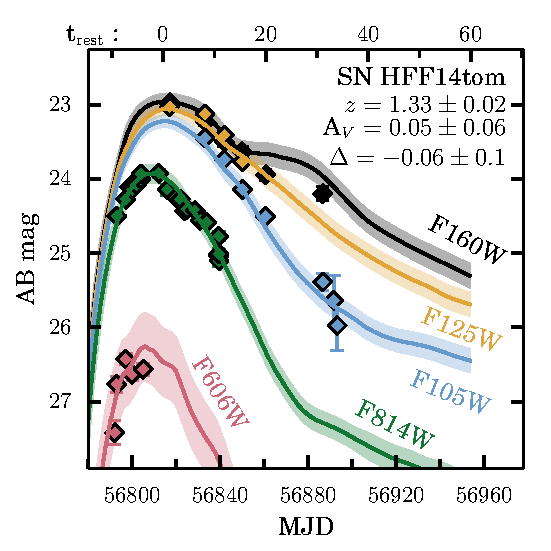
\includegraphics[width=0.49\textwidth]{FIG/lcfit_mlcs2k2_ABmag}
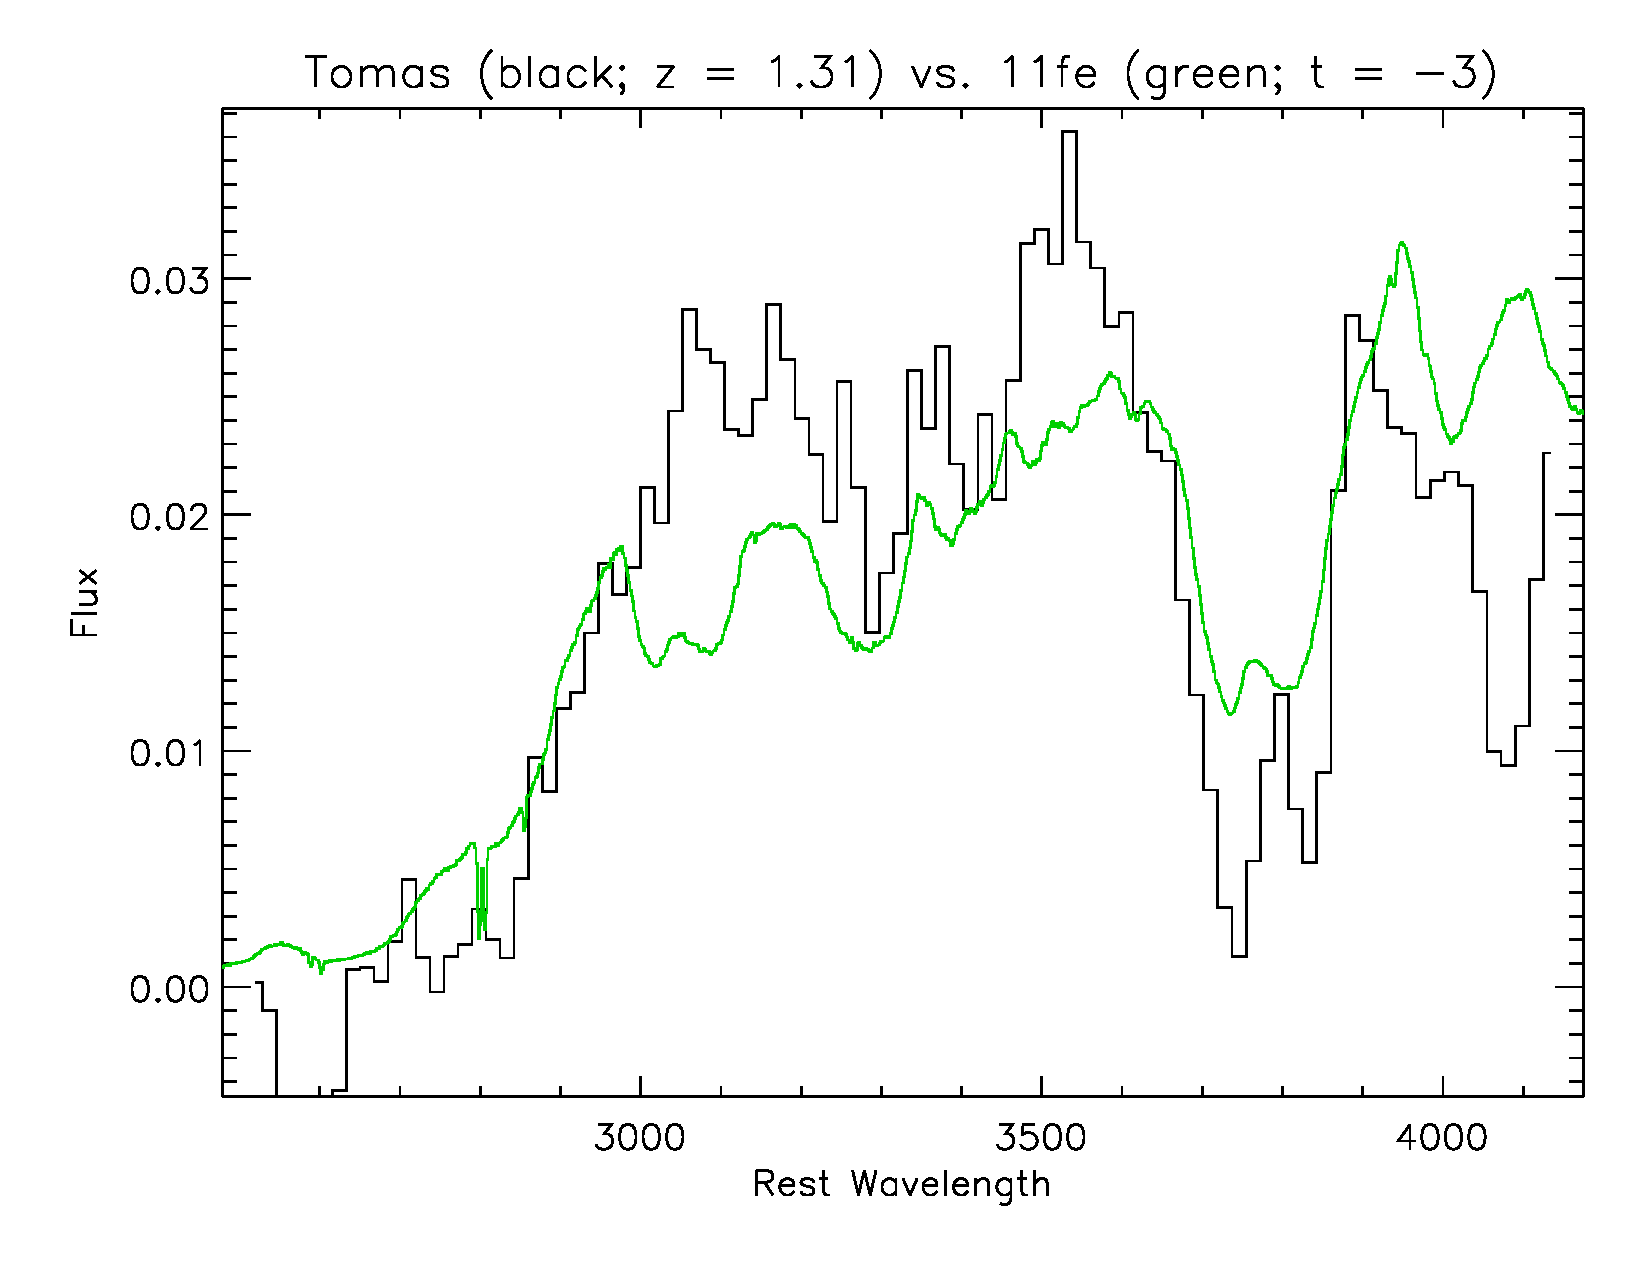
\includegraphics[width=0.49\textwidth]{FIG/specfit_11fe_t-3_z131}
\caption{ {\it (Left)} Light curve fit using MLCS2k2. 
{\it (Right)} Spectral template match to the HST ACS G800L SN
spectrum.  Assuming minimal reddening, the best-fit template is from
SN 2011fe at $z=1.31$ and $t=-3$ rest-frame days before peak
brightness.  Allowing a correction for the broad SED shape using
3rd-order polynomials, the best match is from SN 2012cg at $z=1.31$
and $t=+3 days$.
\label{fig:mlcsfit} }
\end{center}
\end{figure*}

\section{Lensing Magnification}
\label{sec:LensingMagnification}


\subsection{Direct Magnification Measurement}
\label{sec:DirectMagnificationMeasurement}


\begin{figure}
\begin{center}
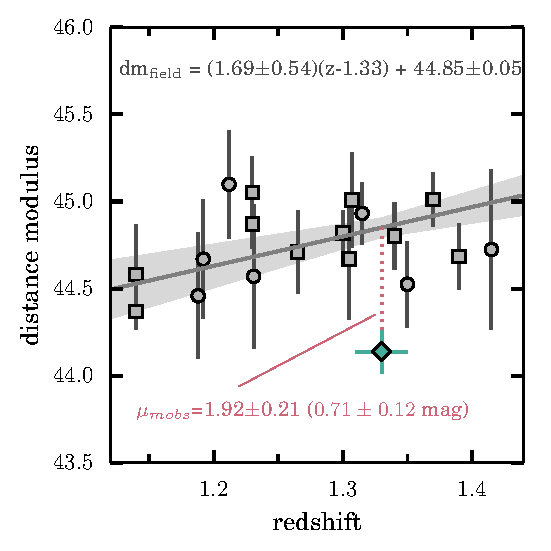
\includegraphics[width=\columnwidth]{FIG/magnification_measurement}
\caption{ Deriving the magnification from comparison to field SN
\label{fig:magmeasure} }
\end{center}
\end{figure}

\subsection{Comparison to Model Predictions}
\label{sec:ComparisonToModelPredictions}


1) All of the lens models predict a higher magnification than we observe, some with discrepancies >5 sigma.  This suggests a systematic bias inherent to all the models -- at least for this particular line of sight. 

2) the addition of new lensing constraints from the HFF data does not reduce the tension.  From both of the most recent models (Jauzac+ 2014 and Lam+ 2014) the predicted magnification is still significantly higher than the observed. 

3) The pre-HFF models that come closest to matching the observed magnification are the Zitrin-NFW and Merten models (also the Williams model, though it has very large uncertainties).  Those happen to be two models that relax or remove the assumption of light-traces-mass.  


\begin{figure}
\begin{center}
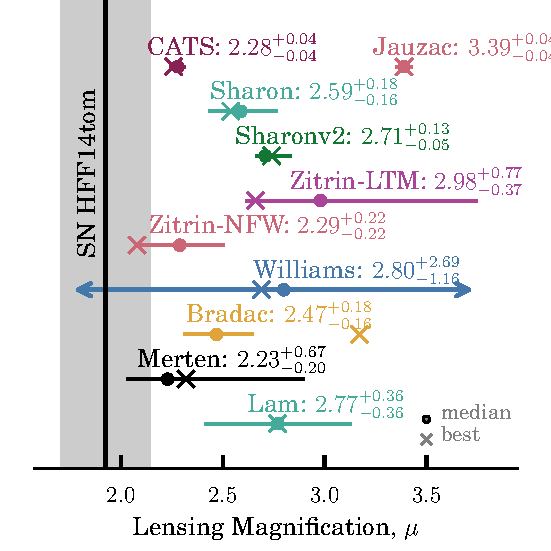
\includegraphics[width=\columnwidth]{FIG/lensing_test}
\caption{ 
Comparison of the observed lensing magnification to predictions from
lens models.
\label{fig:lensingtest} }
\end{center}
\end{figure}


\section{Discussion}

Possible sources for the bias. 

Implications for the systematic error budget of high-z lenses.

Proposal for a survey to build a bigger sample : HST GO, Snapshot, ground-based.

\bigskip


{\bf Acknowledgments:}

We are very pleased to thank the Hubble Frontier Fields team at STScI
for their substantial efforts to make the HFF program successful.  In
particular, thanks are due to Matt Mountain for the allocation of
discretionary orbits for the HFF program; to Jennifer Lotz, Norman
Grogin and Patricia Royle for accommodations in strategy and
implementation to make the FrontierSN program possible; and to Dan Coe
for curating the excellent and accessible lens model comparison tools.
We also must thank the CLASH team, led by Marc Postman, for
observations, catalogs, and high level science products that were of
significant value for this analysis.

Financial support for this work was provided by NASA through grants
HST-HF-51312 and HST-GO-13386 from the Space Telescope
Science Institute, which is operated by Associated Universities for
Research in Astronomy, Inc., under NASA contract NAS 5-26555.  Support
for this research at Rutgers University was provided in part by NSF
CAREER award AST-0847157 to SWJ.  The Dark Cosmology Centre is
supported by the Danish National Research Foundation.


{\it Facilities:} \facility{HST (WFC3)}
\smallskip

\bibliographystyle{apj}
\bibliography{bibdesk}

\end{document}

